\chapter{Systeme}
Betrachtet man die typische Nachrichtenübertragungskette, so ist
das Bindeglied zwischen Quelle und Senke der Kanal. Eine andere
allgmeinere Bezeichnung für den Kanal ist der Begriff System. Ganz
allgemein kann davon gesprochen werden, dass ein System
verschiedene (unterschiedliche) Signale miteinander verknüpft und
Beziehungen herstellt. Abbildung \ref{pic:SystembildAllgemein}
zeigt eine allgemeine Verknüpfung von Signalen.

\begin{figure}[h]
\begin{center}
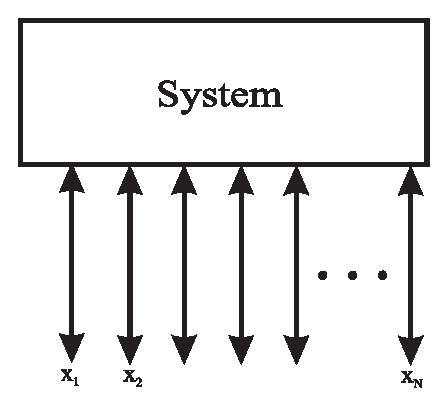
\includegraphics{psSys/SystemAllgemein}
\caption{\label{pic:SystembildAllgemein} Veranschaulichung eines
allgemeinen Systems, dass Signale miteinander verknüpft.}
\end{center}
\end{figure}

In den meisten Fällen, kann diese sehr allgemeine Verknüpfung
spezifiziert werden. Insbesondere haben wir häufig Eingangssignale
auf die das System reagiert und die daraus resultierenden
Ausgangssignale (siehe Abbildung \ref{pic:SystembildEinAus}).

\begin{figure}[H]
\begin{center}
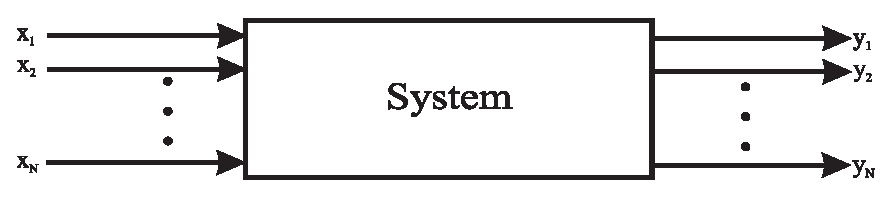
\includegraphics{psSys/SystemEinAus}
\caption{\label{pic:SystembildEinAus} Veranschaulichung eines
allgemeinen Systems, mit Signalen die als Ein- und Ausgangssignale
festliegen.}
\end{center}
\end{figure}

Durch diese sehr allgemeine Formulierung des Systembegriffs wird
auch deutlich, warum die Systemtheorie eine zentraler Punkt vieler
wissenschaftlicher Richtungen ist. Dies wird  auch deutlich, wenn
man einige Beispiele betrachtet:
\begin{itemize}
    \item HiFi-Verstärker: Ein System mit mehreren Eingängen und
    wenigen (meist zwei) Ausgängen
    \item Der Mensch: Ein sehr komplexes System mit vielen
    Eingängen (Sinnesorganen) und vielen Ausgängen (Muskeln)
    \item Computer: Viele Eingänge und Ausgänge
    \item Ihr Beispiel
\end{itemize}


\section{Eigenschaften und Klassifikation von Systemen}
Bei der Klassifikation der Systeme, können wir zunächst die
meisten Punkte, die wir für Signale erarbeitet haben, ebenfalls
anwenden.
\subsection{Wert- und Definitionsbereich}
Da wären zunächst die Frage, ob es sich bei dem betrachteten
System um ein analoges (wertkontinuierlich und zeitkontinuierlich)
oder um ein digitales (zeit- und wertdiskret) System  handelt. In
den nächsten Abschnitten werden wir uns zunächst nur mit digitalen
Systemen beschäftigen.

Die Klassifikation erfolgt also nach:

\wichtig{analoges System vs. digitales System}

\subsection{Kanalanzahl}
Die Kanalanzahl ist ebenfalls eine Möglichkeit ein System zu
beschreiben und zu klassifizieren, wobei als Besonderheit zu
beachten ist, dass Systeme auch die Kanalanzahl verändern können.
So kann \zB ein Monosignal (Gesang) auf zwei Kanäle aufgespalten
werden um so eine Positionierung in einem Stereosignal zu
ermöglichen.

\begin{figure}[H]
\begin{center}
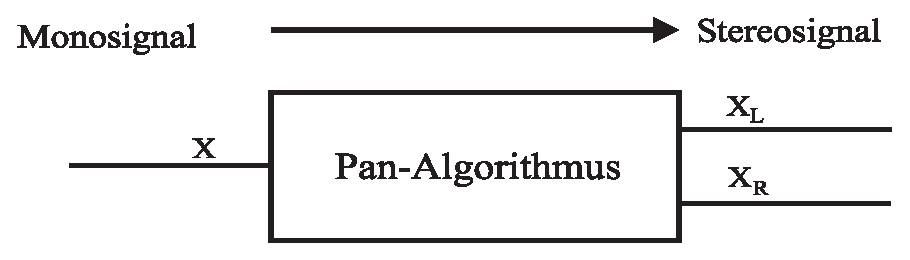
\includegraphics[width = 10cm]{psSys/PanAllgemein}
\caption{\label{pic:PanAlgo} Beispiel eines Systems mit einem
Eingang und zwei Ausgängen.}
\end{center}
\end{figure}

Wir können also Systeme nach der Kanalzahl der Ein- und Ausgänge
klassifizieren.

\wichtig{Einkanalig vs. Mehrkanalig}

Der allgemeinste Fall des mehrkanaligen Ein- und Ausgangs wird
als MIMO {\em Multiple Input Multiple Output} System bezeichnet.

\subsection{Dimensionalität}
So wie es ein- und mehrdimensionale Signale gibt, so können auch
Systeme in mehreren Dimensionen wirken. Ein einfaches Beispiel
wäre ein bildveränderndes System, dass natürlich zwei-dimensional
arbeiten müsste.

\wichtig{eindimensional vs. mehrdimensional}


\subsection{Rekursivität \label{ssec:Rekursion}}
Eine Eigenschaft, die wir bisher nicht mit Signalen erarbeitet
haben, ist die Frage, ob das System den eigenen Ausgang als
weiteren Eingang betrachtet. Abbildung \ref{pic:RekursivSystem}
zeigt ein System
dass sein Ausgangssignal auf den Eingang zurückführt. Ein solches
System bezeichnen wir als rekursives System.

\begin{figure}[H]
\begin{center}
\includegraphics[width = 10cm]{psSys/RekursivSystem}
\caption{\label{pic:RekursivSystem} Allgemeines Blockdiagramm
eines einkanaligen rekursiven Systems.}
\end{center}
\end{figure}

Da es auch nicht-rekursive Systeme gibt, können wir folgende
Klassifikation einführen

\wichtig {rekursive vs. nicht-rekursive (transversal) Systeme }

Um die Wichtigkeit von rekursiven Systemen zu verdeutlichen,
nehmen wir einmal an, wir bräuchten ständig die Summe von mehreren
vergangenen Messwerten (oder ein Beispiel aus der Praxis ist der
30-Tage Durchschnitt bei der DAX-Analyse). Wir können diese Summe
immer wieder durch folgende Formel berechnen. Die Anzahl der
Messwerte, die wir verwenden ist durch $M$ symbolisiert.
\begin{equation}
y(k) = \sum_{m=0}^{M-1}x(k-m)
\end{equation}

Betrachtet man diese Rechenvorschrift, so fällt auf, dass
bestimmte Anteile immer wieder summiert werden und immer nur ein
neuer Wert hinzukommt und ein alter Wert herausfällt aus der
Summation. Dies ist in Abbildung \ref{pic:ErklaerungRekursion}
genauer gezeigt.

\begin{figure}[H]
\begin{center}
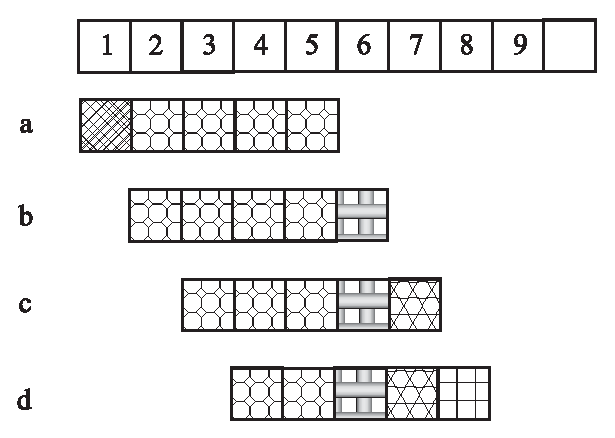
\includegraphics[width = 8cm]{psSys/DatenwerteRekursion}
\caption{\label{pic:ErklaerungRekursion} Erläuterung zur Anwendung
der Rekursion. Bei einer Summenbildung über die jeweiligen Zeilen
(a-d) sind die Summen zwischen a und b die achteckig gefüllten
Elemente bereits für a addiert worden. Man kann deshalb bei b
durch Subtraktion des gestrichelten ersten Elements und Addition
des Elements mit Kreuz direkt die neue Summe berechnen.}
\end{center}
\end{figure}

Man könnte also das Ausgangssignal des Systems auch durch folgende
Rechenvorschrift berechnen
\begin{equation} \label{eq:RekursionsBsp}
    y(k) = y(k-1) + x(k) - x(k-(M)).
\end{equation}

Es ist also möglich die Rechenleistung durch rekursive
Berechnungen zu verringern.

\subsection{Gedächtnis}
Bei der Rekursion haben wir gesehen, dass durch Speicherung der
Eingangsfolge und Speicherung des letzten Ausgangswertes sehr
einfach bestimmte Systeme realisiert werden können. Systeme die
Speicherelemente beinhalten werden gedächtnisbehaftet genannt.
Systeme bei denen der Ausgang nur von den Eingangssignalen, aber
nicht von dem vorherigen Zustand abhängig ist, sind gedächtnislos.
Ein Beispiel für ein gedächtnisloses System ist die Funktion $y(k)
= x^2(k)$.

\wichtig{Gedächtnisbehaftet vs. Gedächtnislos}

Die Gedächtnislänge eines Systems ist
durch die Möglichkeit der größten Signalverzögerung $k_0$
vorgegeben. Diese kann im transversalen oder im rekursiven Zweig
des Systems vorkommen. Der Hauptunterschied liegt im Einfluss des Gedächtnisses.
Bei ausschließlich transversalen Systemen bestimmt die Gedächtnislänge die
Einflusslänge. Für rekursive Systeme ist die Einflusslänge bis auf sehr wenige Ausnahmen unabhängig
von der Gedächtnislänge unendlich.

\subsection{Kausalität}
Die Kausalität ist für Systeme eine sehr wichtige Eigenschaft. Nur
bei kausalen Systemen ist die Ursache (Eingangssignal) zeitlich
immer vor der Wirkung (Ausgangssignal). Anders ausgedrückt das
Ausgangssignal darf nur von dem jetztigen Eingang und vorherigen
Eingangswerten abhängen, damit ein kausales System vorliegt.
Mathematisch kann dies durch
\begin{equation}
    y(k_0) = f\{x(k\leq k_0)\}
\end{equation}
ausgedrückt werden.

\subsection{Stabilität}
Eine andere sehr wichtige Eigenschaft für Systeme ist ihre
Stabilität. Stabile Systeme zeichnen sich dadurch aus, dass sie
auf ein begrenztes Eingangssignal mit einem begrenzten
Ausgangssignal reagieren (BIBO-Stabilität (Bounded input bounded
output)) Mathematisch muss folgendes als notwendige Bedingung gelten:
\begin{equation}
\mbox{wenn} \quad |x(k)| < \infty \quad \Rightarrow \quad |f\{x(k)\}| <
\infty
\end{equation}
\begin{example}
Sind die folgenden Systeme stabil?
\begin{itemize}
    \item $y(k) = x^2(k)$:\\
    Das System ist stabil, da alle möglichen Eingangswerte für
    x(k), die kleiner als $|\infty|$ sind, wieder auf Werte führen
    die kleiner als $\infty$ sind
    \item $y(k) = \log(x(k))$:\\
    Für $x(k) = 0$ ist $y(k) = -\infty$. Somit ist das System
    instabil.
\end{itemize}
\end{example}

\section{LTI-Systeme}
Eine besondere Klasse an Systemen stellen die linearen,
zeitinvarianten (LTI: linear and time-invariant) Systeme dar. Die
beiden Begriffe Linearität und Zeit-invarianz werden im weiteren
als Systemeigenschaften genauer beschrieben

\subsection{Linearität}
Lineare Systeme zeichnen sich dadurch aus, dass das sog.
Superpositionsprinzip (Überlagerungsprinzip) gilt. Dies bedeutet,
dass die additive Überlagerung der gewichteten Eingangssignale und
die Verknüpfung mit dem System genau zu dem gleichen Ergebnis
führt, wie die gewichtete additive Überlagerung der einzelnen
Signale am Ausgang des linearen Systems. Mathematisch ausgedrückt:
\begin{equation} \label{eq:Linearitaet}
    f\{a_1 x_1(k) + a_2 x_2(k) + \cdots + a_N x_N(k)\} = a_1 f\{x_1(k)\} + a_2 f\{x_2(k)\} + \cdots + a_N f\{x_N(k)\}
\end{equation}
wobei $f\{\cdot\}$ die Systemfunktion darstellt, $a_i$ die
linearen Gewichte und $x_i(k)$ die Eingangssignale. Abbildung
\ref{eq:Linearitaet} verdeutlicht den mathematischen Zusammenhang noch einmal
grafisch. Bei LTI-Systemen kann das System $H$ vor den Summationspunkt und vor
den linearen Gewichten $a_1$ und $a_2$ verschoben werden.

\begin{figure}[H]
\begin{center}
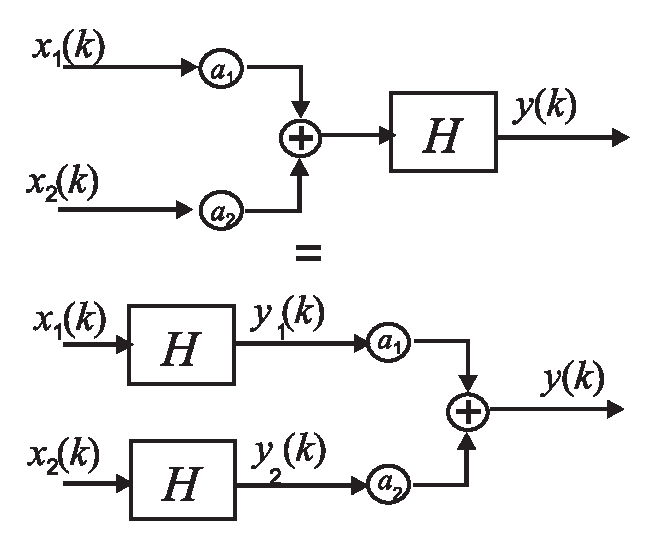
\includegraphics[width = 10cm]{psSys/LinearitaetErklaerung}
\caption{\label{pic:Linearitaet} Linearität bildlich erklärt}
\end{center}
\end{figure}

\begin{example}
Als Beispiel betrachten wir das System
\begin{equation}
y(k) = 2x(k) + 3x(k-1)
\end{equation}

Der Ausgang der einzelnen Eingangssignale $x_1(k)$ und $x_2(k)$
gewichtet ergeben.
\begin{eqnarray}
y_1(k) &= & (2x_1(k) + 3x_1(k-1))\\
y_2(k) &= & (2x_2(k) + 3x_2(k-1))\\
\end{eqnarray}
Der Ausgang ergibt sich zu
\begin{equation}\label{eq:Ausgangdirekt}
y(k) = a_1 y_1(k)+ a_2 y_2(k).
\end{equation}
und somit
\begin{equation}\label{eq:AusgangdirektFinal}
y(k) = 2 a_1  x_1(k) + 3 a_1 x_1(k-1)+  2 a_2 x_2(k) + 3 a_2 x_2(k-1) .
\end{equation}

Ein gemischtes und gewichtetes Eingangssignal ist gegeben durch
\begin{equation}
x_{mix} = a_1 x_1(k) + a_2 x_2(k)
\end{equation}
und das Ausgangssignal des System durch
\begin{eqnarray}
y(k) &=& 2x_{mix}(k) + 3x_{mix}(k-1)\\\nonumber
& = & 2(a_1 x_1(k) + a_2 x_2(k)) + 3(a_1 x_1(k-1) + a_2 x_2(k-1))\\\nonumber
& = & 2a_1x_1(k) + 2 a_2 x_2(k) + 3 a_1 x_1(k-1) + 3 a_2 x_2(k-1)
\end{eqnarray}
Dies ist im Vergleich zur Gleichung \ref{eq:Ausgangdirekt}
identisch. Somit ist das System linear.

Als zweites System testen wir $y(k) = x^2(k)$. Es ergeben sich
folgende Ausgangssignale:
\begin{eqnarray}
y_1(k) & = & x_1^2 (k)\\
y_2(k) & = & x_2^2 (k)\\
\Rightarrow y(k) &= &a_1 y_1(k) + a_2 y_2(k)\\
& = & a_1  x_1^2 (k) + a_2  x_2^2 (k)
\end{eqnarray}
bzw.
\begin{eqnarray}
y(k) &= &  x_{mix}^2 (k)\\
& = & \left( a_1  x_1 (k) + a_2  x_2 (k) \right)^2\\
 & = & a_1^2 x_1^2 (k) + 2a_1 a_2 x_1(k) x_2(k) + a_2^2 x_2^2 (k)
\end{eqnarray}
Die beiden Ausgangssignale sind nicht identisch. Dieses System ist
also nicht-linear.
\end{example}

\subsection{Zeit-Invarianz}
Von Zeitinvarianz spricht man, wenn das System seine Eigenschaften
nicht zeitlich ändert. Eine bestimmmte Verzögerung $k_0$ des
Eingangssignal führt also im Ausgang zu einem um die selbe Zeit
$k_0$ verzögerten Ausgangssignal. Mathematisch ausgedrückt:
\begin{equation}
y(k) = f\{x(k) \} \quad \Rightarrow y(k-k_0) = f\{x(k-k_0) \}
\end{equation}
mit $k_0$ als Angabe der diskreten Verzögerungszeit.

\begin{example}
Gegeben sind die beiden Systeme $y(k) = 2x(k)$ und $y(k) = x(2k)$.
Sind die Systeme zeitinvariant oder nicht?

Der Test erfolgt zum einen über die zeitliche Verschiebung des
Eingangssignal $x(k)$. Es ergibt sich ein neues Eingangssignal
$x(k-k_0)$. Für dieses neue Eingangssignal ist der Ausgang $y(k) =
2x(k-k_0)$. Zum anderen muss das Ausgangssignal des
Originaleingangssignals verschoben werden. Es ergibt sich zunächst
für den Ausgang $y(k) = 2 x(k)$. Dieses Signal wird jetzt um $k_0$
verschoben (Variablensubstitution $k' = k-k_0$). Der Ausgang ist
also $y(k') = y(k-k_0) = 2 x(k-k_0)$. Das System ist
zeit-invariant.

Beim zweiten System ergibt sich am Ausgang durch die Verschiebung
des Eingangssignals $y(k) = x(2k-k_0)$. Betrachtet man aber den um
$k_0$ verschobenen Ausgang ergibt sich durch die
Variablensubstitution $y(k-k_0) = x(2k-2k_0)$. Dieses System ist
also zeitvariant.
\end{example}


\subsection{Beschreibung durch Differenzengleichungen}
LTI-Systeme lassen sich stets durch Differenzengleichungen mit
festen Koeffizienten ausdrücken. Dies ist für nicht-rekursive
Systeme mit den Beispielen des Abschnittes über Linearität auch
leicht nachvollziehbar. Gleichzeitig gilt die selbe
Linearitätsbeziehung auch für den Ausgang des Systems. Betrachtet
man nun ein System, dass rekursiv ist, so kommen als neue Terme
nur vergangene Systemantworten mit linearen Faktoren gewichtet
(multipliziert) hinzu. Damit sind auch alle durch folgende
Gleichung aufgebauten rekursiven Systeme linear.
\begin{equation}
\sum_{i = 0}^{N} a_i y(k-i) = \sum_{j = 0}^{M}b_j x(k-j)
\end{equation}
Um nun nur den Ausgang des Systems zu betrachten, wird vereinbart,
dass $a_0 = 1$ ist\footnote{Dies könnte jederzeit durch eine
Division durch $a_0$ erreicht werden.}. Für den Ausgang eines
kausalen Systems gilt dann
\begin{equation}
y(k) = -\sum_{i = 1}^{N}a_i y(k-i) + \sum_{j = 0}^{M}b_j
x(k-j)
\end{equation}

%Die Summe für die rekursiven Signalanteile beginnt bei 1, da der
%0. Koeffizient eigentlich dem aktuellem Ausgangssignal zugeordnet
%ist, so wie $b_0$ dem aktuellen Eingangswert zugeordnet ist. Da
%wir aber eine ungewichtete Ausgangsfolge haben wollen, wird $a_0$
%auf eins normiert. Ist dieser Wert bei einer gegebenen Aufgabe
%ungleich null, so müssen alle Koeffizienten $a_i$ und $b_j$ durch
%$a_0$ dividiert werden.

Um zu wissen, welche Folge $y(k)$ am Ausgang herauskommt, ist es
notwendig den aktuellen und die vergangenen Eingangssignale $x(k)$
zu kennen. Zusätzlich muss aber auch bekannt sein, wie die inneren
Zustände des Systems aussehen. Es müssen also die vorherigen
Ausgangswerte bekannt sein, um die vollständige Beschreibung zu
gewährleisten. Häufig wird vereinfacht angenommen, dass das System
in Ruhe war und deshalb gilt
\[
   y(k-i) = 0 \qquad \forall \qquad i>0.
\]

\subsubsection{Einführung der Systemantwort auf die Delta-Impulsfolge}
Die Systemantwort auf die Delta-Impulsfolge $\delta(k)$ wird als
Impulsantwort $h(k)$ bezeichnet und charakterisiert ein LTI-System
vollständig. Für nicht-rekursive Systeme mit einer endlichen
Anzahl von Koeffizienten, also $M< \infty$ ist die Impulsantwort
endlich. Deshalb werden diese Systeme auch als {\em Finite Impulse
Response} (FIR)-Systeme bezeichnet. Bei rekursiven Systeme gilt
dies im allgemeinen nicht. Diese Systeme werden im
englischsprachigen Raum, deshalb als {\em Infinite Impulse
Response} (IIR)-Systeme bezeichnet.

\begin{example}

Nehmen wir an, wir suchen die Impulsantwort des LTI-Systems $y(k)
= r_0 x(k) + r_1 x(k-1) - r_2 x(k-2)$. Errechnet man nun den
Ausgang für alle $k$ und setzt jeweils für x(k) die Impulsfolge
ein, so ergibt sich die Impulsantwort\footnote{Die Impulsantwort wird hier
in einer Vektorschreibweise eingeführt.} $h(k) = [r_0 \,\, r_1 \,\,
-r_2]$ für $0 \leq k \leq 2$. Das betrachtete System
war ein FIR-System. Ganz allgemein ergibt sich für FIR-Systeme
immer, dass $h(k) = b_k$ ist.

Für IIR-Systeme ist die Berechnung der Impulsantwort nicht so
trivial. Betrachten wir das System
\[
y(k) = \alpha y(k-1) + \beta x(k).
\]
Als Eingangssignal nutzen wir erneut $x(k)= \delta(k)$.
Die Ausgangsfolge für
alle $k$ berechnet, ergibt
\[h(k) = [\beta \,\, \alpha \beta \,\,
\alpha \alpha \beta \,\, \cdots \,\, \alpha^{k}\beta].
\]
Die Impulsantwort endet nicht.
\end{example}

Für viele Probleme reicht es aber aus, die Impulsantwort nur so
weit zu betrachten, wie sich noch signifikante Werte ergeben.
Signifikant kann dabei zum Beispiel sein zu testen, ob die Werte
von $h(k)$ kleiner als der millionste Teil des maximalen Wertes
von $h(k)$ ist.

\wichtig{Die Impulsantwort eines Systems ist der Ausgang des
Systems, wenn die Eingangsfolge die Delta-Impulsfolge ist. Die
Impulsantwort beschreibt ein LTI-System vollständig}

\wichtig{Nicht-rekursive Systeme haben eine endliche Impulsantwort.
Sie werden als FIR-Systeme bezeichnet.}

\subsection{Faltung als Verknüpfung von LTI-Systemen und Signalen}
Bisher haben wir nur gesehen, wie die Eingangssignale durch die
Differenzengleichung zum Ausgangssignal werden. Es gibt aber eine
allgemeinere Vorschrift, die direkt mit der Impulsantwort zusammen
hängt.

Zur Veranschaulichung wird zunächst ein einfaches Beispiel berechnet.
Das Eingangssignal ist
durch zwei Werte gegeben, wir nehmen an $x(0)= 0.5$ und $x(1) =
1.5$. Das System ist durch $y(k) = -0.25x(k) + 0.5x(k-1)$
definiert. Wie lautet die Ausgangssfolge? Man könnte jetzt einfach
die verschiedenen Zeitpunkte $k$ annehmen und das Ergebnis direkt
hinschreiben. In Tabellenform wäre das Ergebnis:

\begin{center}
\begin{tabular}{|c|c|c|c|}\hline
$k$ & $x(k)$ & $x(k-1)$ & $y(k)$ \\\hline
0 & 0.5 & 0   & -0.125\\ \hline
1 & 1.5 & 0.5 & -0.125\\ \hline
2 &  0  & 1.5 &  0.75\\ \hline
3 &  0  &  0  &    0\\ \hline
\end{tabular}
\end{center}

Für dieses einfache Beispiel ist das noch leicht möglich, bei längeren Folgen
wäre diese Lösung unpraktisch.
Statt dessen versuchen wir einen allgemeineren
Lösungsweg zu finden. Die Eingangsfolge $x(k)$ lässt sich für alle $k$
mit Hilfe der delta-Folge $\delta(k)$ durch
\begin{equation}\label{eq:diracinput}
    x(k) = 0.5 \delta(k) +  1.5 \delta(k-1)
\end{equation}
vollständig beschreiben.

Mit dem Gesetz der Linearität und dem Wissen der Impulsantwort
$h(k) = [-0.25 \:\, 0.5]$, ergibt sich die Antwort für $y(k)$ aus
der Summe der gewichteten und verschobenen Impulsantworten, da
jede der delta-Folgen die Impulsantwort als Systemantwort hervor
ruft.

Allgemeiner lässt sich sagen, jedes diskrete Eingangssignal lässt
sich in viele kleine Einzelimpulse zerlegen. Wir haben es also
immer mit einer gewichteten Summe von Delta-Impulsfolgen zu tun.
Aus dem letzten Abschnitt haben wir kennengelernt, dass die
Impulsantwort ein LTI-System vollständig beschreibt. Außerdem gilt
für LTI-Systeme das Superpositionsprinzip. Das Ausgangssignal
eines LTI-Systems kann deshalb durch eine mit linearen
Koeffizienten gewichtete Addition der zeitlich verschobenen
Impulsantwort berechnet werden.

Um dies zu veranschaulichen, ist in Abbildung
\ref{pic:Faltungserklaerung} diese Zerlegung für ein Beispiel
durchgeführt. Bild a) zeigt die Eingangssfolge $x(k) = [1\,\, 0.5
\,\, 1]$ , Bild b) das System $h = [0.5 \,\,\,  0.75 \; 1]$.
Zerlegt man nun die Eingangsfolge in drei Einzelimpulse ergeben
sich die drei Bilder c,e,g. Jeder dieser Einzelimpulse erzeugt
eine verschobene und gewichtete Version der Impulsantwort (Bild
d,f,h). Das Ausgangssignal (i) ergibt sich schlussendlich aus der
Summe dieser Ausgangssignale.
\begin{figure}[H]
\begin{center}
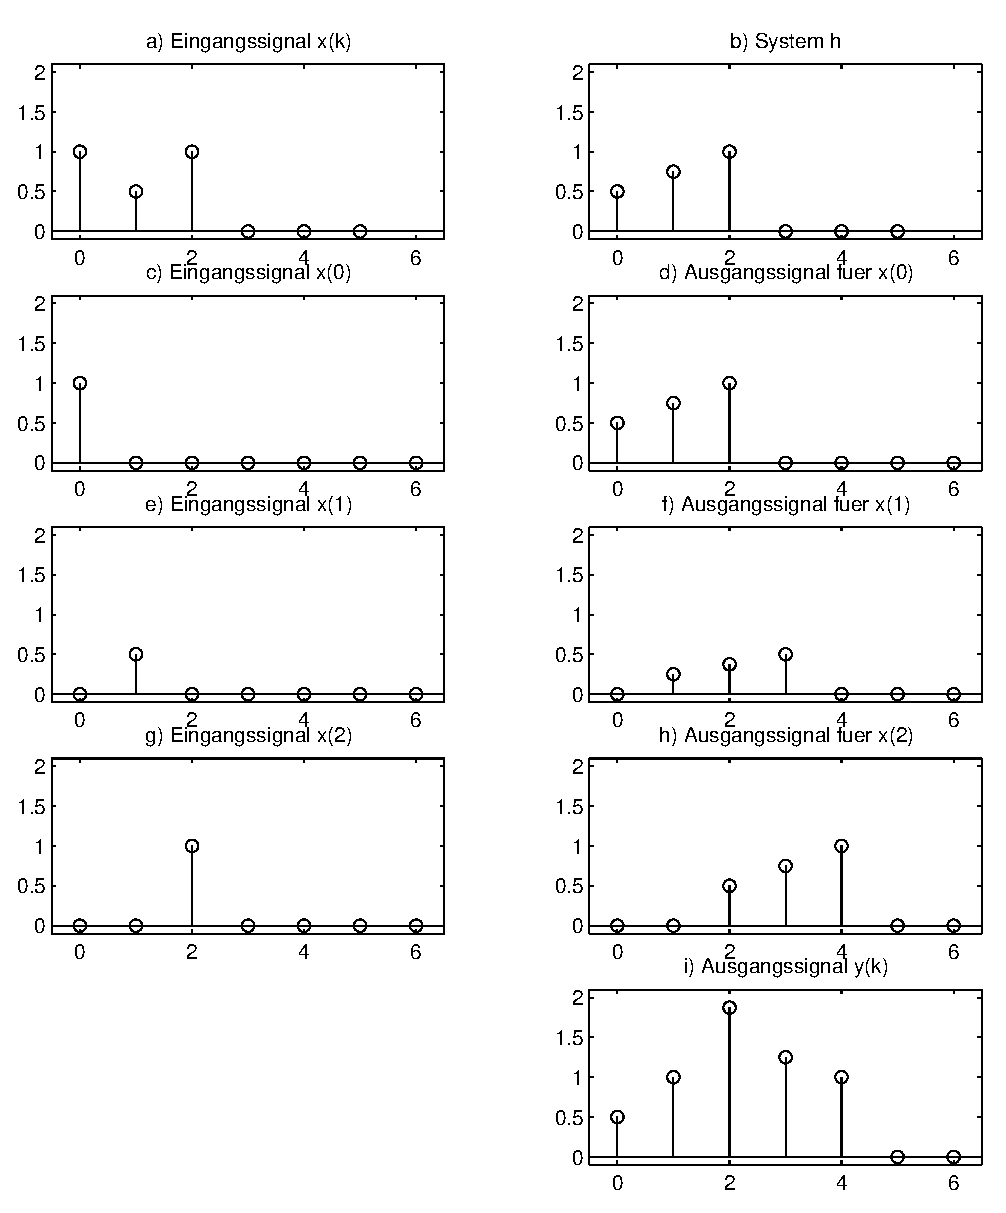
\includegraphics[width = 16cm]{psSys/FaltungErklaerung}
\caption{\label{pic:Faltungserklaerung} Einfache grafische
Erklärung der Faltung}
\end{center}
\end{figure}

Allgemein und mathematisch wird dies durch
\begin{equation}
    y(k) = \sum_{\kappa = -\infty}^{\infty} h(\kappa) x(k-\kappa)
\end{equation}
ausgedrückt. Diese Summe wird als Symbol durch $\ast$ dargestellt und als
Faltungsumme bezeichnet:
\begin{eqnarray}
    y(k) &=& \sum_{\kappa = -\infty}^{\infty} h(\kappa) x(k-\kappa)\\
        & = & h(k) \ast x(k)
\end{eqnarray}

\subsubsection{Eigenschaften der Faltung}
Der Faltungsoperator ($\ast$) kann wie die Multiplikation aufgefasst werden.
Es gelten die folgenden mathematische Gesetze:
\begin{itemize}
\item Kommutativgesetz
\begin{equation}\label{eq:FaltungKommu}
    x(k) \ast h(k) = h(k) \ast x(k)
\end{equation}
\item Assoziativgesetz
\begin{equation}\label{eq:FaltungAssoz}
   ( x(k) \ast y(k)) \ast h(k) =  x(k) \ast (y(k) \ast h(k))
\end{equation}
\item Distributivgesetz
\begin{equation}\label{eq:FaltungDistrib}
   ( x(k) + y(k)) \ast h(k) =  x(k)\ast h(k) +  y(k) \ast h(k)
\end{equation}


\end{itemize}

\subsubsection{grafische Faltung}
Die Berechnung des Faltungsproduktes lässt sich auch grafisch gut
veranschaulichen. Dazu betrachten wir Abbildung
\ref{pic:GraphischeFaltungErk}. Die beiden zu faltenden Folgen $x(k)$
und $h(k)$ sind in a) gezeigt. Das Faltungsergebnis erhält man,
wenn man eine der Folgen zeitlich spiegelt b), also an der y-Achse
umklappt und diese Folge über das andere Signal schiebt c). Der
Ausgang d) ergibt sich immer aus der Summe der sich überlappenden
und miteinander multiplizierten Einzelimpulse der beiden Folgen.

\begin{figure}[H]
\begin{center}
\includegraphics[width = 12cm]{psSys/FaltungsErklaerungCorel}
\caption{\label{pic:GraphischeFaltungErk} Erklärung der grafischen
Faltung}
\end{center}
\end{figure}

Die Länge der Ausgangsfolge ergibt sich aus der Addition der
Länge der Eingangsfolge $M$ und der Länge der Impulsantwort $K$ zu
\begin{equation}
    N = M + K - 1.
\end{equation}
Dies ist auch anhand der beiden grafischen Beispiele
leicht zu sehen.

\tbd{grafische Faltung bei analogen Signalen}

\compileif{bBook}
{
\section{Systeme und Matlab}
Auch hier gilt, siehe Script.
\subsection{Test auf Nicht-Linearität und Zeitvarianz}
\subsection{Faltung}
}

\section{Übungen}
\subsection{Wiederholung des Stoffes und einfache Rechenaufgaben}
\begin{enumerate}
    \item Ist ein Quantisierer ein lineares System, da ja von
    linearer Quantisierung gesprochen wird? Begründen Sie ihr
    Antwort.
    \item Sind die folgenden Systeme zeitinvariant, kausal und linear? Begründen Sie ihre Antwort.
    \begin{itemize}
        \item{$y(k) = x(k) + 2d $ mit $d\neq 0$}
        \item $y(k) = a_1 x(k-2) + a_2 x(k-3)$
        \item $y(k) = k x(k-1) + x(k-2)$
        \item $y(k) = log_{10}( x(k-2)) + 3 x(k-1) $
    \end{itemize}
    \item Falten Sie die folgenden vier Signale jeweils grafisch mit sich selbst und mit allen anderen
    Signalen.
    \begin{figure}[H]
    \begin{center}
    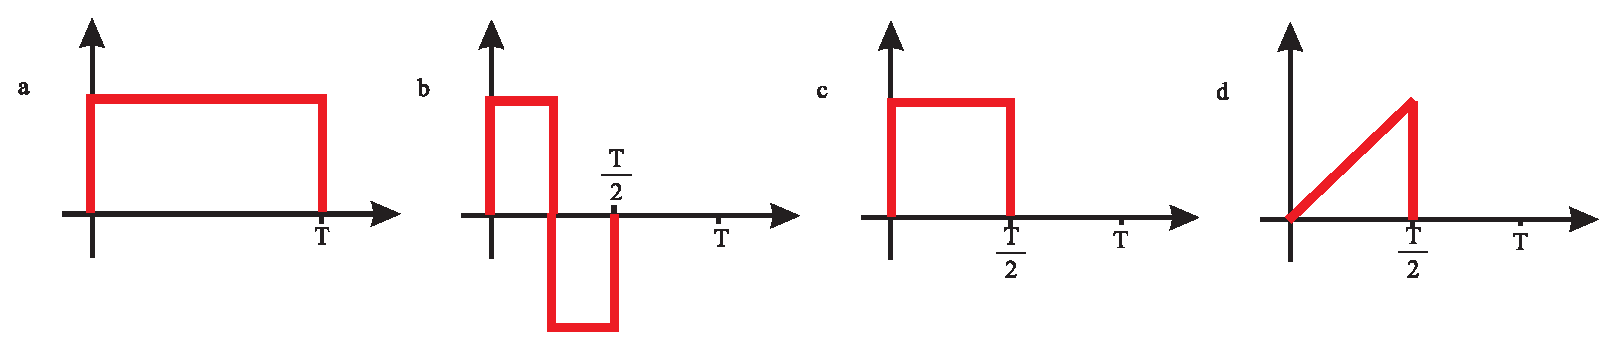
\includegraphics[width = 15cm]{psUeb/GraphikFaltung}
    \caption{\label{pic:UebungGraphischeFaltung}Testsignale zum Üben der grafischen Faltung}
    \end{center}
    \end{figure}
    \item Zeigen Sie, dass das Kommutativgesetz der Faltung allgemein gilt.
\end{enumerate}
\subsection{Aufgaben (Einige auf Klausurniveau)\label{ssec:Aufgaben}}
\begin{enumerate}
    \item \label{Aufg:impulsfolge}Geben sie die Impulsantwort für die folgenden
    Differenzengleichungen an. Brechen
    Sie bei unendlichen Folgen nach $k=10$ ab. Nehmen sie an, dass sich das System zum Zeitpunkt $k=0$
    in Ruhe befand.
    \begin{enumerate}
        \item $y(k) = 0.5x(k-1)+ 0.3x(k-2)+ 0.4x(k-3) - 0.4 x(k-4)$
        \item $y(k) = y(k-1)+0.5x(k)$
        \item $y(k) = 0.25 x(k-1)+0.75 y(k-1) - 0.75y(k-3)$
    \end{enumerate}
    \item Gegeben ist das System $0 = \frac{1}{k} x(k) + 2x(k-2) - 0.5y(k-1)$. Begründen Sie
    Linearität und Zeit-Invarianz bitte mathematisch formal!

    \item
\end{enumerate}

\compileif{bBook}
{
\subsection{Matlab-Aufgaben}
\begin{enumerate}
    \item Testen Sie folgende Systeme auf Zeitinvarianz und Linearität durch Rauschfolgen als
    Eingangssignale. Haben Sie im Hinterkopf, dass Sie mit Zahlentests nichts beweisen können.
    Eine Aussage ist nur für Nicht-Linearität und Zeitvarianz möglich. Dies ergibt sich, wenn
    der Test fehl schlägt, da {\em ein} Gegenbeispiel ausreicht um Linearität oder Zeitinvarianz
    auszuschließen.
    \begin{itemize}
        \item $y(k) = x(k) + y(k-1)$
        \item $y(k) = 3 y(k-1) + 2 x(k-1) + x(k)$
        \item $y(k) = k x(k-1) + x(k-2)$
        \item $y(k) = log_{10} x(k-2) + 3 y(k-1) $
    \end{itemize}
    \item Erzeugen Sie eine Funktion die eine Delta-Impulsfolge mit vordefinierter Länge zurück gibt.
    \item Nutzen Sie diese Funktion, um ihre Ergebnisse aus Abschnitt \ref{ssec:Aufgaben} Aufgabe \ref{Aufg:impulsfolge} zu überprüfen.
    \item Erzeugen Sie kurze Sequenzen mit $T = 12$ Werten um die oben gezeigten Signale zu approximieren.
    Überprüfen Sie Ihre Ergebnisse mit dem {\tt conv}-Befehl.
\end{enumerate}
}
\subsection{Transfer-Leistung}
\begin{enumerate}
    \item
    \item
    \item
\end{enumerate}
%
\compileif{bZusammenfassung}
{
\section{Zusammenfassung}
Die wichtigen Erkenntnisse aus diesem Kapitel sind:
\begin{itemize}
    \item Lineare zeitinvariante (LTI)-Systeme stellen eine wichitge Klasse der Systeme dar.
    \item LTI-Systeme lassen sich vollständig durch Differenzengleichungen beschreiben.
    \item Die Faltung verknüpft LTI-Systeme und Signale
    \item Die Impulsantwort ist das Ausgangssignal eines Systems, wenn die Delta-Folge als
    Eingang gewählt wurde. Sie beschreibt ein LTI-System ebenfalls vollständig.
\end{itemize}
}
%\newpage

%\section{Lösungen zu den Übungsaufgaben}
